\section{Research methodology}

The development process from Heath et al.~\cite{heath2009survey} (figure~\ref{fig:steps_simulation}) will be followed.

\subsection{Problem formulation and setting of the objectives}
This part is done in the research questions part.





The initial basic requirements of this model are:

\begin{itemize}
    \item   The world consists op a grid of squares, some squares will be blocks of buildings and others represent the streets.
    \item   On this grid some predetermined restaurants and customers exist.
    \item   Customers will order food at a restaurant, the restaurant will prepare the food en will ask for a deliverer.
    \item   A deliverer will claim the delivery, move to the restaurant, pick the food up and move to the customer.
    \item   Agents may leave the world, i.e.,choose another delivery company, when unhappy.
    \item   Unhappiness will occur:
    \begin{itemize}
        \item   for customers when the food is not or too late delivered,
        \item   for restaurants when the food is not picked up or no orders are being placed,
        \item   for deliverers when they don't make any money.
    \end{itemize}
    \item    Calculating the profit for the delivery company.
    \item    The simulation consists of discreet steps, in which all agents simultaneous can do one thing.
    Some examples are:
    \begin{itemize}
        \item  move to the next square
        \item  place an order at a restaurant
        \item  do nothing
        \item  decide to take an order
    \end{itemize}
    \item   Behavior of the agents is rule based, these have to be programmed.
\end{itemize}

More requirements will be found during development, and some will be dropped.

To summarize the design problem: to improve insight into profitability in whether to employ deliverers,
an ABM will be created in NetLogo that replicates a real world food delivery situation and satisfies the above-listed requirements,
so that stakeholders, including the author, can use this to make an unbiased analysis.




The research methodology consists of creating an Agent Based Model in NetLogo, deciding the behaviour rules of the agents and program them in the model, conduct
experiments by running simulations in which different variables are set.

The model details, and result will be presented in a paper.

The model based approach is a way to eliminate all variables not direct related to the problem and keep only the essence of the situation.
Also, a real world experiment is not possible, at least not for a single researcher.

The environment where multiple agents act is called a multi-agent system end the problem is called a multi-agent planning problem (from~\cite{russell2016artificial}).
The research problem is actually a comparison between a system where there is one decision maker (the company assigns delivery jobs) and a system where each deliverer decide for its self (multiple decision makers).
This research will not be of a thoroughly theoretical nature though, its more of an exploratory/explanatory nature, see what happens under some conditions and explain the correlation.

The nature of a NetLogo model is that in each step, a time unit, all actors do something (or do nothing) but the order in which the actors do something is random.
There is an interleaved execution of events, no race conditions take place, this solves the problem of who gets a delivery job in case of several free deliverers.

An effort will be made to search for existing NetLogo models that can be reused.

First example: a grid with roads is used in the Taxi Cab model~\cite{dongpingtaxicabs2019} as shown in figure~\ref{fig:taxi cab}
\begin{figure}
    \centering
    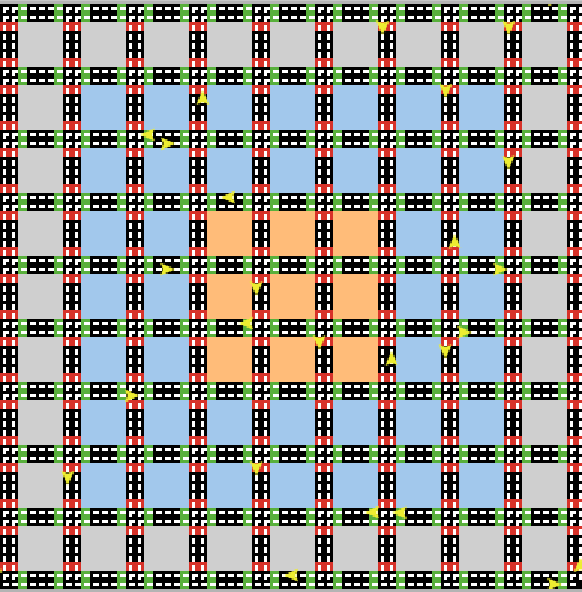
\includegraphics[width=6cm]{sections/pics/Taxi Cabs}
    \caption{Taxi Cab Model}
    \label{fig:taxi cab}
\end{figure}

Second example: the simulation is used in ~\cite{ismail2024software}.
In this study some rules, goals and tasks are listed, shown in figure~\ref{fig:tasktable} , that can be adapted and used in our model.
The NetLogo ui of this model is shown in figure~\ref{fig:a-ride}.
\begin{figure}
    \centering
    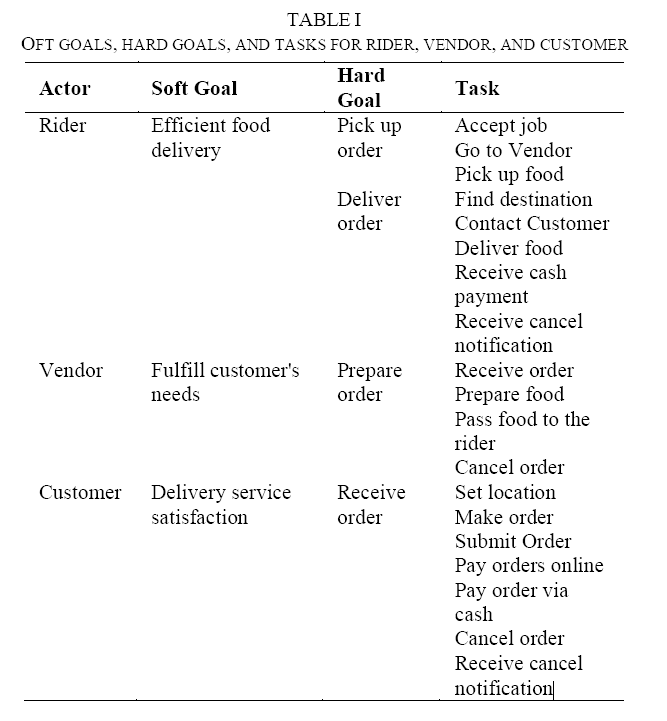
\includegraphics[width=8cm]{sections/pics/TaskTabel}
    \caption{Food Delivery}
    \label{fig:tasktable}
\end{figure}

\begin{figure*}
    \centering
    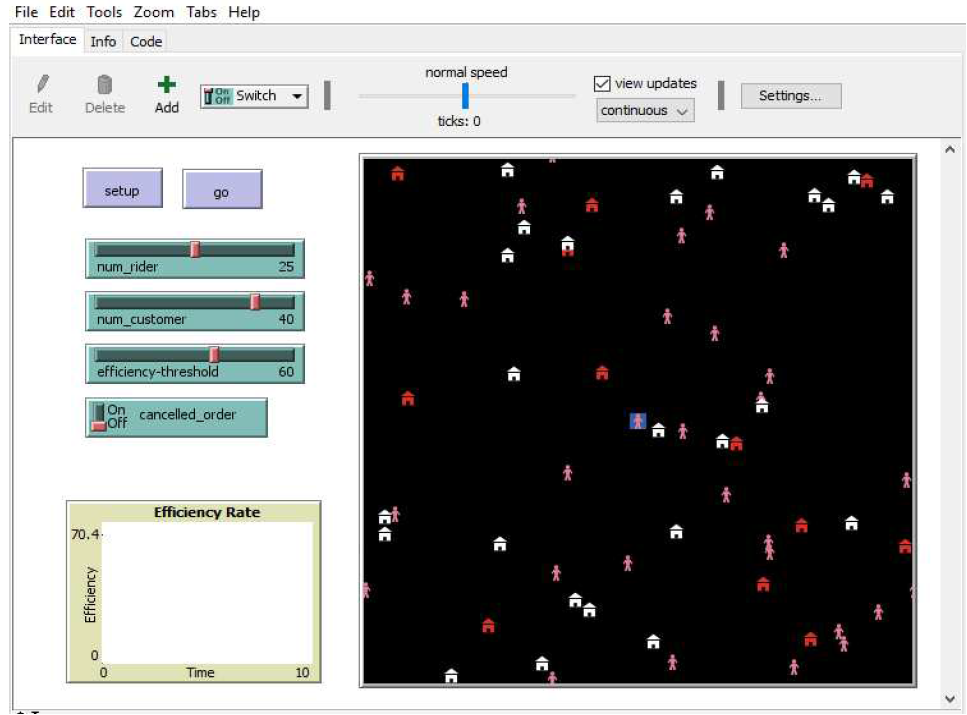
\includegraphics[width=\linewidth]{sections/pics/a-ride}
    \caption{NetLogo a-ride simulation}
    \label{fig:a-ride}
\end{figure*}
